\documentclass[../main.tex]{subfiles}
\graphicspath{{./images/}}
\begin{document}
\section{Discussion}

Here we will look at how to add images into our document. Every folder for each chapter has its own images file where you will upload graphics for your project, additionally, each tex file has packages for adding these images to your document and manipulating them. 

Here when using the begin{figure} command, we write it as begin{figure}[H], this specified the position of the figure to start where you have started the figure in the text as opposed to just floating about and doing what it wanted.

\begin{figure}[H]
    \centering
    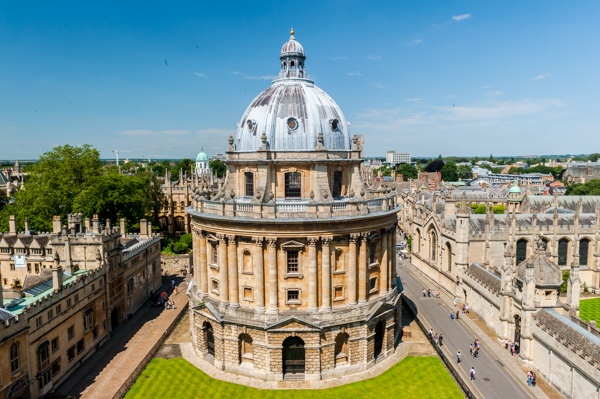
\includegraphics[width=0.5\linewidth]{Chapter5/images/Radcliffe-Camera-8163.jpg}
    \caption{A lovely shot of the radcliffe camera taken from 
    \href{https://www.britainexpress.com/cities/oxford/radcliffe.htm}{Britain express}}
    \label{fig:enter-label}
\end{figure}

We can change the size and the scaling of the image using the commands shown:

\begin{figure}[H]
    \centering
    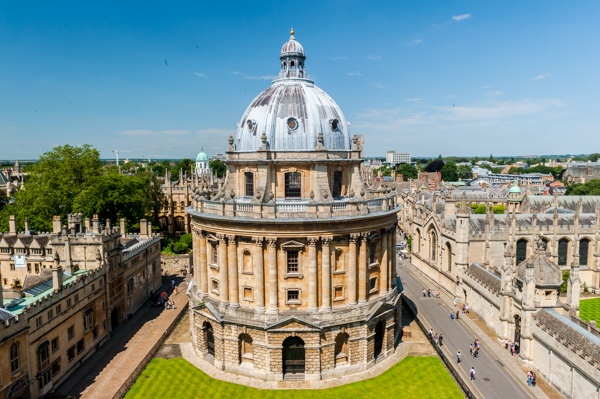
\includegraphics[width=0.9\linewidth]{Chapter5/images/Radcliffe-Camera-8163.jpg}
    \caption{A lovely shot of the Radcliffe camera, this time BIG. The default for the figure captions is to write from center and then when one line is complete, fill from the right. This can be changed if you prefer it to be from the right or left using the raggedright or other packages, I wouldn't bother as is more effort than its worth and honestly looks no better}
    \label{fig:enter-label}
\end{figure}

\begin{figure}[H]
    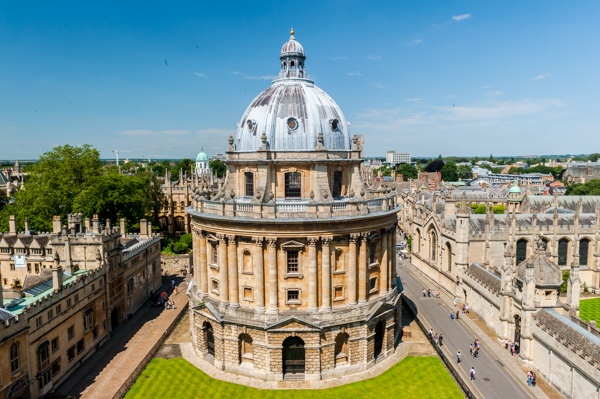
\includegraphics[width=0.3\linewidth,left]{Chapter5/images/Radcliffe-Camera-8163.jpg}
    \caption{A lovely shot of the Radcliffe camera, this time on the left}
    \label{fig:enter-label}
\end{figure}
\begin{figure}[H]
    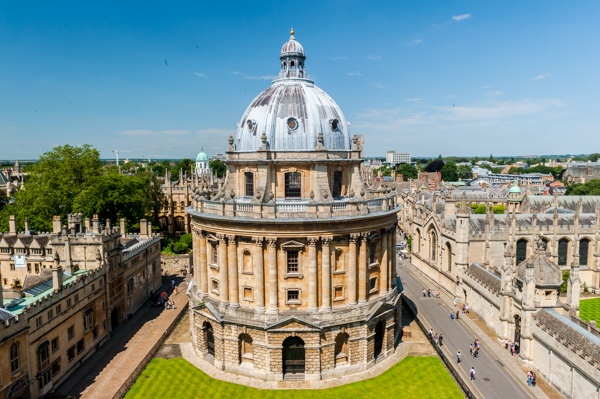
\includegraphics[width=0.3\linewidth,right]{Chapter5/images/Radcliffe-Camera-8163.jpg}
    \caption{A lovely shot of the Radcliffe camera this time on the right}
    \label{fig:enter-label}
\end{figure}


\end{document}